\section{Results}
\label{sec:results}

The results show a visibility-to-curatability funnel. Public records often support discovery and collection organization, but the record set narrows as curation requires stronger combinations of evidence: 90.7\% of analysis-set paper records are discovery-ready; 18.1\% combine usable provenance with concrete code, recipe, or stronger release evidence; and 6.1\% additionally satisfy the high-curatability requirement of direct linkage plus asset-level or multi-asset release evidence. Table~\ref{tab:key-results} summarizes the evidence ingredients and composite thresholds. The five RQs follow the curation workflow. RQ1--RQ4 explain why identity, linkage, provenance, and release evidence each exist in public records but cannot be substituted for one another; RQ5 diagnoses where these fields fail to co-occur.

\begin{table*}[!tbp]
\centering
\caption{Headline evidence components and curation thresholds. Counts use 2,214 analysis-set paper records. $P$, $R$, and $L$ denote provenance, release-package, and direct-linkage scores.}
\label{tab:key-results}
\normalsize
\setlength{\tabcolsep}{6pt}
\renewcommand{\arraystretch}{1.08}
\begin{tabular*}{\textwidth}{@{\extracolsep{\fill}}llrrl@{}}
\toprule
\textbf{Group} & \textbf{Evidence or threshold} & \textbf{Count} & \textbf{Share} & \textbf{Takeaway} \\
\midrule
\multicolumn{5}{@{}l}{\textit{Evidence components}} \\
\cmidrule(lr){1-5}
Linkage & Matched paper--HF repo & 124 / 2,214 & 5.6\% & Direct relation rare \\
Provenance & Inventory-backed family & 1,009 / 2,214 & 45.6\% & Grouping, not lineage \\
Release & Code/asset evidence ($R\geq2$) & 793 / 2,214 & 35.8\% & Concrete release uneven \\
\midrule
\multicolumn{5}{@{}l}{\textit{Curation-readiness thresholds}} \\
\cmidrule(lr){1-5}
Discovery-ready & Any useful signal & 2,008 / 2,214 & \textbf{90.7\%} & Broad visibility \\
Operational P+R & $P\geq2, R\geq2$ & 401 / 2,214 & \textbf{18.1\%} & Usable P + release \\
High-curatability & $P\geq2, R\geq3, L\geq1$ & 136 / 2,214 & \textbf{6.1\%} & Joint evidence bottleneck \\
Preservation-review & $P\geq2, R\geq4, L\geq1$ & 50 / 2,214 & 2.3\% & Multi-asset subset \\
\bottomrule
\end{tabular*}
\renewcommand{\arraystretch}{1.0}
\end{table*}


\subsection{RQ1: Can Repository Records Identify Artifact Roles?}

Repository records provide broad coverage for artifact typing, but confidence is uneven across roles. In the fixed \hf snapshot, our pipeline assigns project-inferred artifact-role and package-form labels to all 191,375 repository records from public metadata and tags. Figure~\ref{fig:metadata}a shows which curation fields are broadly visible and which remain sparse: task descriptors, family labels, upstream fields, and license signals appear frequently, while scholarly references and domain descriptors remain much less complete. Figure~\ref{fig:metadata}b shows that role typing is stable for several derived-artifact classes, while base and merge/mixed records require richer package-form information.

\begin{figure*}[!tbp]
    \centering
    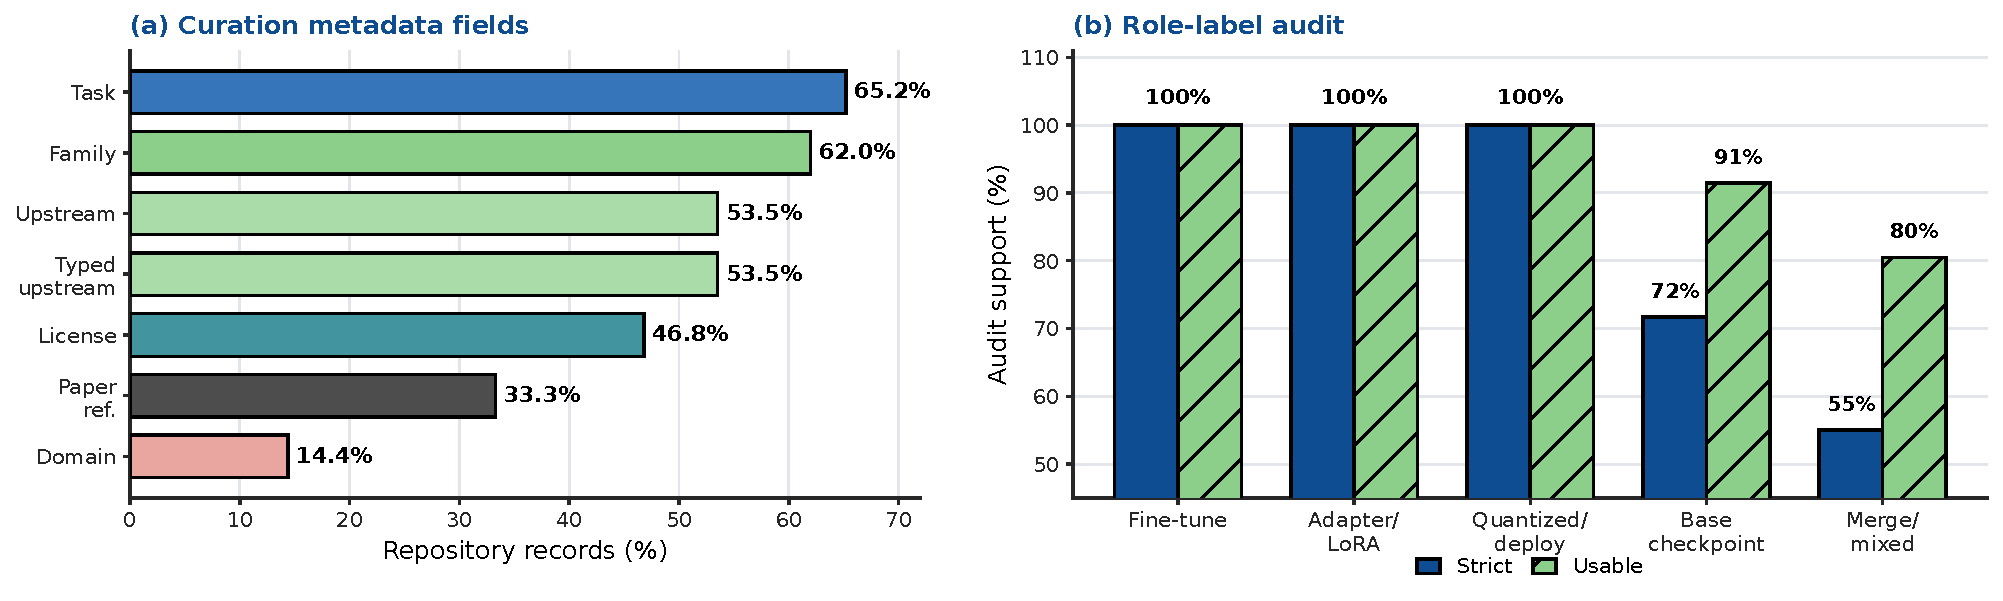
\includegraphics[width=\textwidth]{figures/fig2_metadata_completeness.pdf}
    \caption{Repository-side metadata coverage and role audit. Panel (a) reports curation-relevant metadata-field coverage across the fixed repository snapshot. Panel (b) shows balanced-audit support for role labels, separating strict support from usable support. Fine-tune, adapter, and quantized/deployment labels are stable in the audit sample; base and merge/mixed labels have lower strict support and wider ambiguity gaps.}
    \Description{A two-panel figure. The first panel is a horizontal bar chart of metadata-field coverage in repository records. The second panel is a grouped vertical bar chart comparing strict and usable audit support for five artifact-role labels.}
    \label{fig:metadata}
\end{figure*}

The balanced 300-repository expert audit finds 85.3\% overall strict role support (256/300; Wilson 95\% CI [80.9, 88.9]). Fine-tune, adapter/LoRA, and quantized/deployment records each reach 100.0\% strict support in the balanced sample (60/60 per class; lower Wilson bound 94.0\%). Base records have 71.7\% strict support (43/60; CI [59.2, 81.5]), and merge/mixed records have 55.0\% strict support (33/60; CI [42.5, 66.9]). These boundary classes are difficult because a repository can simultaneously carry base-family, merge, converted, or deployment signals; a single generic model label cannot capture that package structure.

For curation, the result is not that every repository has a single unambiguous identity. It is that public metadata can support a first typing layer if catalogs preserve both the primary artifact role and the package form, rather than collapsing base checkpoints, adapters, quantized files, merged models, and deployment packages into one generic model label. The next question is whether those typed repository records can be connected to the papers that introduce, use, or evaluate them.

\subsection{RQ2: What Bibliographic and Linkage Evidence Is Visible?}

The linkage break occurs between visible links and typed scholarly relations. GitHub or code-hosting links appear in 30.6\% of analysis-set paper records and \hf links in 10.5\%, yet matched paper-to-\hf repository evidence covers only 124 of 2,214 records, or 5.6\%. The problem is therefore not the absence of any link, but that links often lack a relation type: official release, dependency, baseline, example, or background reference.

Repository-side fields provide supporting context for linkage and discovery. Across the full snapshot, task descriptors appear in 65.2\% of repository records, model-family labels in 62.0\%, explicit upstream model fields in 53.5\%, typed upstream relation fields in 53.5\%, license tag signals in 46.8\%, scholarly references in 33.3\%, and domain descriptors in 14.4\%. These fields help organize a model collection, but they do not by themselves establish whether a repository is the artifact introduced by a paper, a dependency used by it, or a baseline cited for comparison.

The curation implication is that paper--repository relations should be typed. A record needs to distinguish whether a repository is introduced by the paper, used as a dependency, evaluated as a baseline, cited as background, or provided as an official release package. Once the relation is located, the next curation question is whether the public record also supports an upstream provenance claim.

\subsection{RQ3: What Level of Provenance Can Public Records Support?}

Public records often support family-level collection organization, while exact upstream claims require typed relation evidence. Figure~\ref{fig:provenance} separates upstream-evidence tiers from paper--repository alignment signals. Panel (a) shows that this pattern holds across mechanisms: exact matched paper--\hf anchors are consistently rare, while inventory-backed or weak family evidence is much more common. Panel (b) decomposes direct alignment signals used for bibliographic linkage; these signals are not treated as provenance unless the linked record exposes an upstream relation.

\begin{figure*}[!tbp]
    \centering
    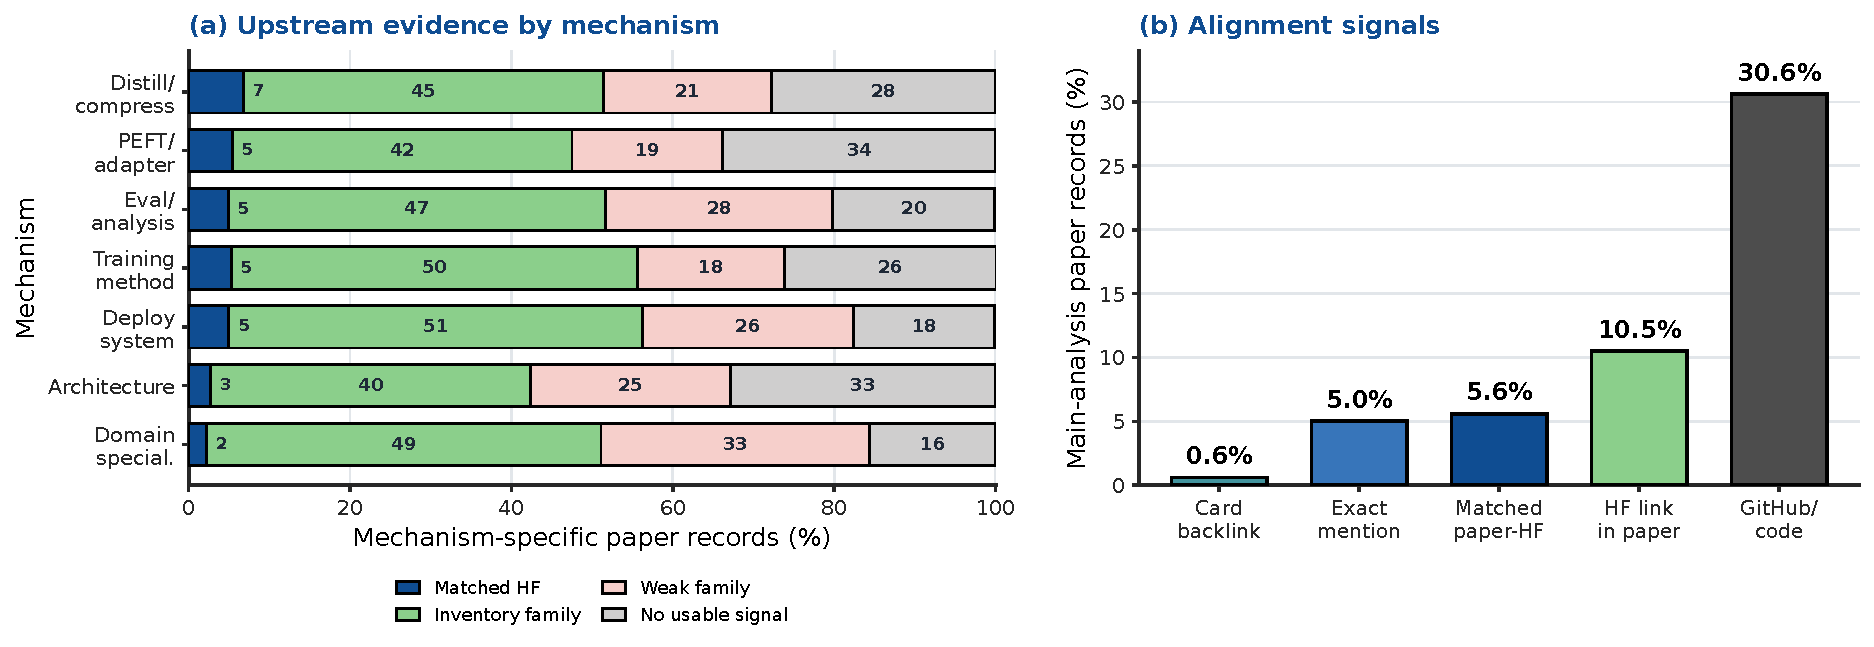
\includegraphics[width=\textwidth]{figures/fig3_provenance_alignment.pdf}
    \caption{Upstream-evidence tiers and paper--repository alignment signals. Panel (a) reports the strongest public-record anchor available for upstream or family-level interpretation by mechanism. Panel (b) ranks direct alignment signals for bibliographic linkage. Alignment signals support provenance only when the linked paper or repository exposes an upstream relation.}
    \Description{A two-panel figure. The first panel is a set of horizontal stacked bars showing upstream and family evidence tiers by research mechanism. The second panel is a vertical bar chart separating paper text links, matched model mentions, model-card backlinks, and the combined matched-link measure.}
    \label{fig:provenance}
\end{figure*}

Inventory-backed family signals cover 45.6\% of analysis-set paper records, weak or contextual family clues cover 21.9\%, and 26.9\% have no usable family or provenance signal. The expert upstream-evidence audit clarifies the strength of these signals: 28.0\% of 200 reviewed rows provide strict evidence for one clear primary upstream family (Wilson 95\% CI [22.2, 34.6]), while 79.0\% provide usable family-level support for collection-level grouping (CI [72.8, 84.1]). In curatorial terms, family evidence is often good enough for shelf placement, but not for a provenance claim.

The result supports a tiered provenance record. Family names are valuable for discovery and aggregate organization, but a curatable record should preserve whether the family appears as a base checkpoint, teacher, adapter target, merge input, quantization source, evaluator, baseline, or only background context. Provenance evidence identifies where an artifact comes from; release evidence determines what part of that artifact can actually be inspected or preserved.

\subsection{RQ4: What Release Package Evidence Is Visible?}

Release evidence is common at the statement level but much rarer at the asset-package level. Figure~\ref{fig:release}a reports the release-package distribution for the 2,214 analysis-set paper records. Overall, 32.8\% have no explicit release signal, 31.3\% have a stated or incomplete release signal, 24.3\% provide code, scripts, or recipe evidence, 6.8\% provide checkpoint or adapter evidence, less than 0.2\% provide data or evaluation asset evidence, and 4.5\% provide multiple assets or a full recipe.

\begin{figure*}[!tbp]
    \centering
    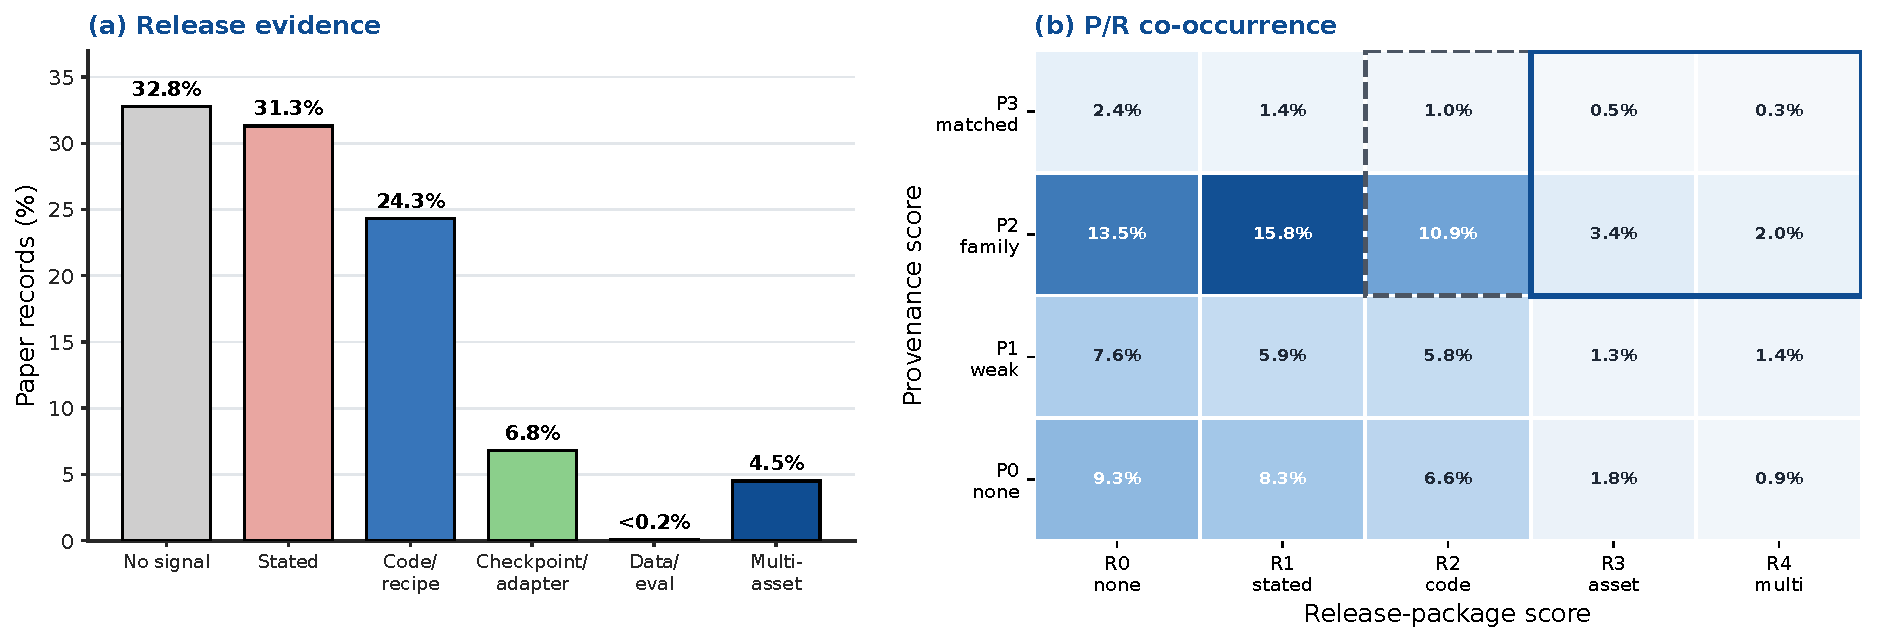
\includegraphics[width=\textwidth]{figures/fig4_release_curatability.pdf}
    \caption{Release evidence and provenance--release co-occurrence. Panel (a) shows release-package evidence by category. Panel (b) cross-tabulates provenance score $P$ and release-package score $R$ for the 2,214 analysis-set paper records; the dashed box marks the operational P+R region and the solid box marks the asset-level region used by the high-curatability threshold.}
    \Description{A two-panel figure. The first panel is a vertical bar chart for release evidence tiers. The second panel is a heatmap crossing provenance scores with release-package scores and highlighting the operational and high-curatability threshold regions.}
    \label{fig:release}
\end{figure*}

Collapsed into broader categories, 67.2\% contain some release or open-asset signal, 35.8\% contain concrete code or asset evidence, and 4.5\% contain strict multi-asset or full-recipe evidence. A targeted 50-row expert URL/asset-level audit found that all reviewed URL/asset assignments matched the visible public-evidence category; no aggregate category changes were required (50/50; Wilson 95\% CI [92.9, 100.0]).

The curation implication is that release should be recorded as a package, not as a binary availability flag. A paper can state that resources are released or expose GitHub scripts while still omitting weights, adapters, data, or evaluation assets; such a record helps inspection but does not yet provide an asset-level package. The final measurement asks how often provenance and release evidence appear together in the same paper record.

\subsection{RQ5: How Often Do the Required Evidence Fields Co-occur?}

The main bottleneck is combined curation readiness. Under the high-curatability threshold, a paper record must have usable provenance, asset-level or multi-asset release evidence, and at least one direct linkage signal. Only 136 of 2,214 analysis-set paper records satisfy this joint-evidence requirement, or 6.1\%.

Table~\ref{tab:key-results} reports the full threshold ladder. A broad discovery-ready rule covers 90.7\% of records. The operational P+R threshold, requiring usable provenance and code/recipe-or-stronger release evidence, covers 18.1\%. The high-curatability threshold covers 6.1\%, and the preservation-review threshold requiring multi-asset or full-recipe evidence covers 2.3\%. Figure~\ref{fig:release}b shows where the drop occurs in the provenance--release co-occurrence map: the operational region with $P\geq2$ and $R\geq2$ contains 401 records, but the asset-level region with $P\geq2$ and $R\geq3$ contains only 136 records.

The key diagnostic is the operational P+R subset. Among 401 records with both usable provenance and concrete release evidence, 400 also contain at least one direct linkage signal. The larger drop from 401 operational P+R records to 136 high-curatability records is therefore driven almost entirely by the release threshold: 265 operational records expose code, scripts, or recipes, but not an asset-level package such as a checkpoint, adapter, data, evaluation asset, or multi-asset recipe. In this corpus, the main bottleneck is not an isolated missing link after provenance and concrete release evidence are present. It is the co-occurrence of usable provenance with sufficiently concrete release assets.

This is the central empirical result: open \llm artifacts are broadly visible, but only a much smaller share expose enough coordinated evidence for provenance-aware curation. The funnel should therefore be read as an evidence-integration problem rather than an artifact-availability problem: the artifacts are often visible, but the record fields needed to justify curation claims are not yet coordinated.
